\documentclass[a4paper,14pt]{extarticle}

\usepackage{amsmath}
\usepackage{amssymb}
\usepackage{amsthm}
\usepackage{fontspec}
\usepackage{polyglossia}
\usepackage[colorlinks=true,urlcolor=black,linkcolor=black,filecolor=black,citecolor=black]{hyperref}
\usepackage{geometry}
\usepackage[style=gost-numeric]{biblatex}
\usepackage{setspace}
\usepackage{lipsum}
\usepackage{caption}
\usepackage{multirow}
\usepackage{pdfpages}
\usepackage{epigraph}

\defaultfontfeatures{Ligatures={TeX}}
\setmainfont{CMU Serif}
\setsansfont{CMU Sans Serif}
\setmonofont{CMU Typewriter Text}

\setdefaultlanguage[spelling=modern]{russian}
\setotherlanguage[variant=british]{english}
\setotherlanguage[variant=classic]{latin}
\frenchspacing
\onehalfspacing

\addbibresource{main.bib}

\newcommand{\ovl}[1]{\overline{#1}}
% For some reason indentfirst doesn't work.
\newcommand{\firstpar}[1]{\hspace{1cm}}

\captionsetup[table]{justification=raggedleft,singlelinecheck=false}
\numberwithin{table}{section}

\theoremstyle{plain}
\newtheorem{rrule}{Правило упрощения}[section]
\newtheorem{brule}[rrule]{Правило расщепления}
\newtheorem{lemma}{Лемма}[section]
\newtheorem{theorem}[lemma]{Теорема}

\theoremstyle{remark}
\newtheorem*{note}{Замечание}

\theoremstyle{definition}
\newtheorem{definition}{Определение}[section]

\title{Новый алгоритм для задачи выполнения наибольшего количества дизъюнктов}
\author{Алфёров Василий Викторович}

\begin{document}
 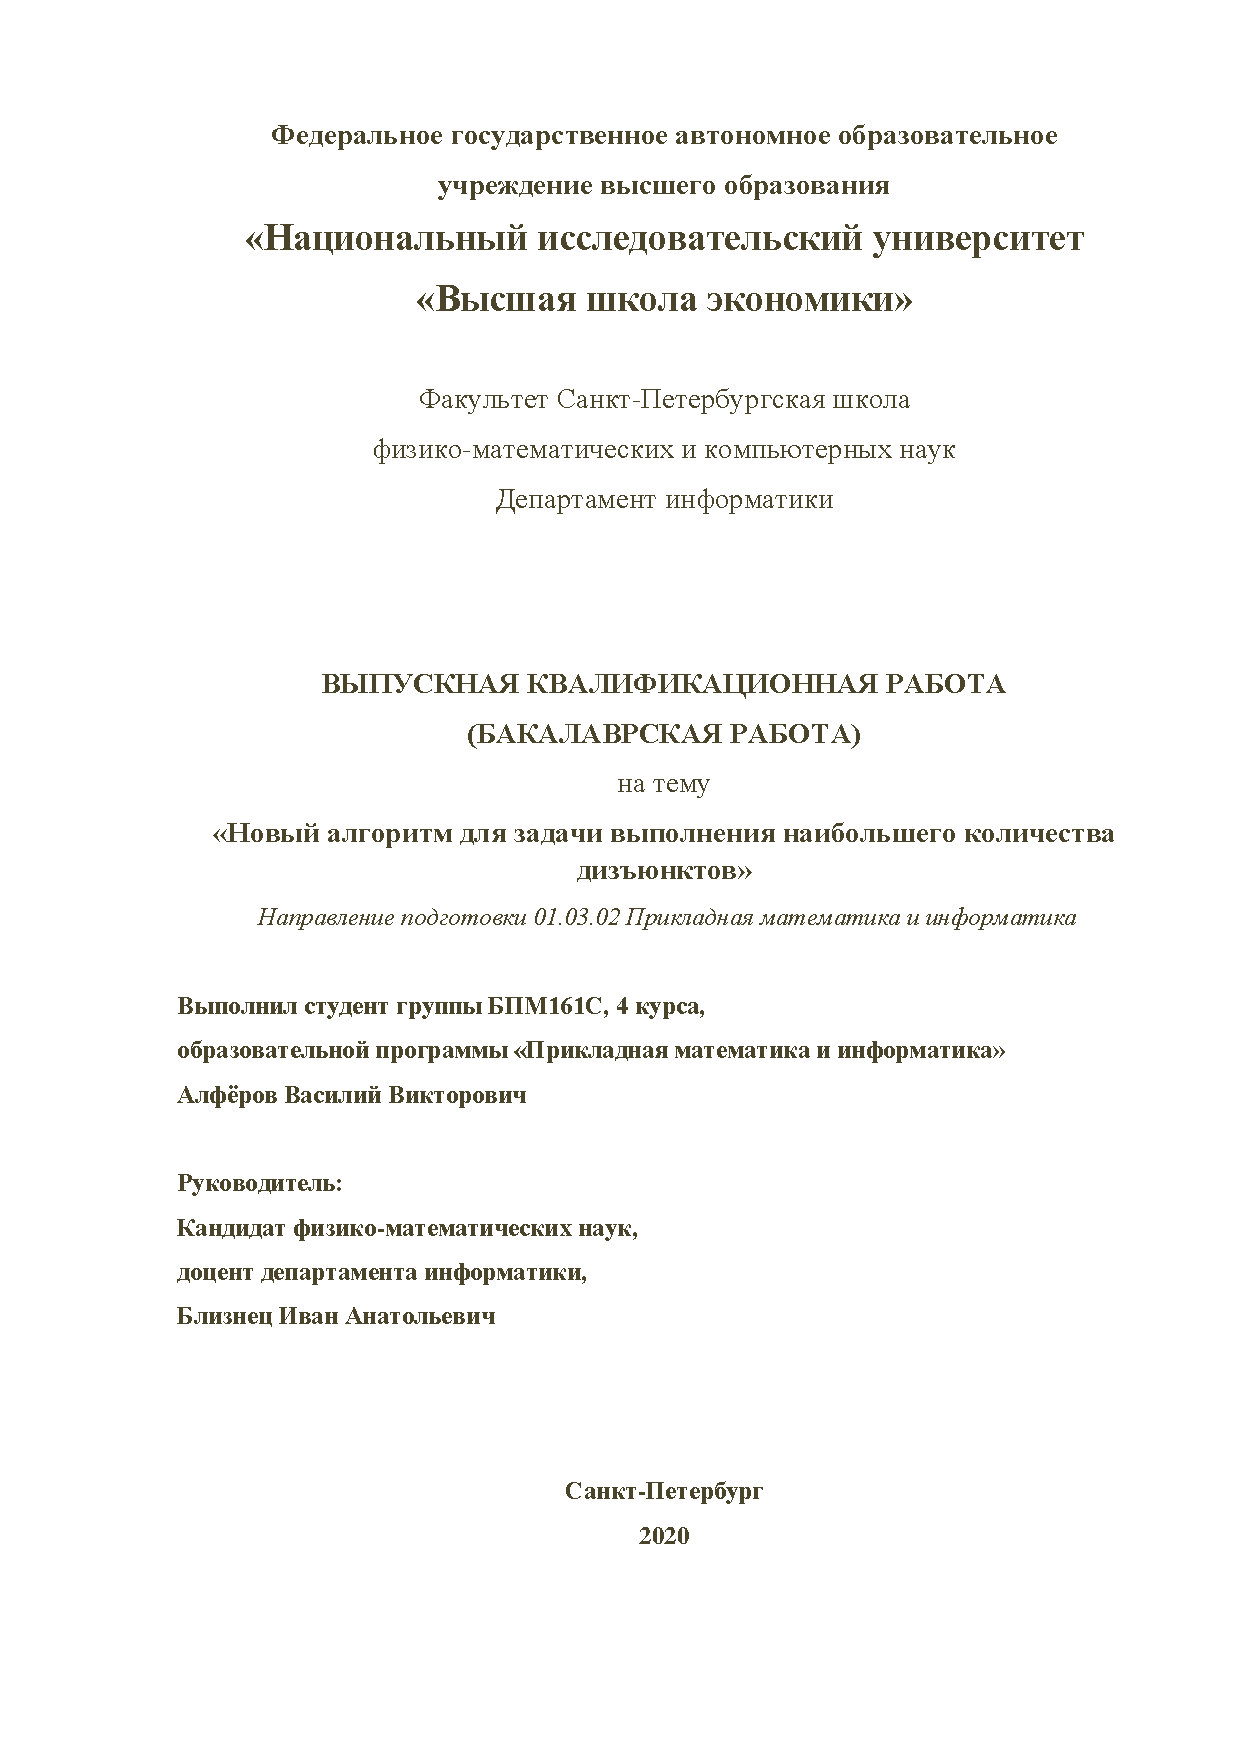
\includepdf{titlepage.pdf}

 \newgeometry{top=2cm,bottom=2cm,left=3cm,right=1.5cm,nohead,includeheadfoot}
\renewcommand{\contentsname}{Оглавление}
\tableofcontents

% vim: spell spelllang=ru_yo,en_gb


 \setlength{\parindent}{1cm}

 \newgeometry{top=2cm,bottom=2cm,left=3cm,right=1.5cm,nohead,includeheadfoot}

\section*{Аннотация}
\label{sec:annotation}
\addcontentsline{toc}{section}{\nameref{sec:annotation}}

\firstpar{}Задача булевой разрешимости -- исторически первая задача, для которой была доказана NP-полнота. Её оптимизационная версия, задача максимальной разрешимости, состоящая в выполнении наибольшего количества дизъюнктов в булевой формуле, также является NP-полной. Несмотря на то, что в предположении гипотезы об экспоненциальном времени эти задачи не могут быть решены за субэкспоненциальное время, задача максимальной разрешимости имеет большое количество применений, и подходы к этой задаче активно изучаются. В последние годы исследования версий задачи максимальной разрешимости, параметризованных общим количеством дизэюнктов и количеством выполненных дизъюнктов, сильно продвинулись за счёт введения сильных правил редукции, основанных на правиле резолюции, и новых техник сведения экземпляра задачи к экземпляру задачи о покрытии множества. Другой важный результат заключаетсчя в том, что задача $(n,3)$-MAXSAT, параметризованная количеством переменных, решается гораздо быстрее, чем в общем случае \cite{belova18}. В данной работе рассматривается задача максимальной разрешимости, решаемая относительно длины формулы, то есть суммарного количества литералов во всех дизъюнктах. Несмотря на то, что некоторые новые правила оказываются полезными для такой задачи, большинство из них увеличивают длину формулы и не могут быть применены. В этой работе представлены новые правила редукции, не увеличивающие длину формулы. Также предлагается новый параметр с пониженной стоимостью 3-переменных, использующий то, что $(n,3)$-MAXSAT решается гораздо быстрее, чем общий случай задачи максимальной разрешимости. Комбинация двух методов позволяет получить алгоритм, работающий за время $O^*(1.093^L)$. Это улучшает предыдущую верхнюю оценку в $O^*(1.106^L)$, полученную Банзалом и Раманом \cite{bansal99}.

\vspace{14pt}

\textit{Ключевые слова:} задача максимальной разрешимости, параметризованные алгоритмы, точные экспоненциальные алгоритмы

\newpage

\begin{otherlanguage}{english}
 Satisfiability problem is historically the first problem that was proven to be NP-complete. Maximum Satisfiability, being its optimization version, is also NP-complete. Though under assumption of Exponential Time Hypothesis those problems cannot be solved in subexponential time, Maximum Satisfiability have many applications, so approaches to solve its instances are nevertheless heavily studied. In the last years, research for versions of Maximum Satisfiability parameterized by the total number of clauses and the number of satisfied clauses have been pushed forward by introducing powerful resolution-based reduction rules and new techniques to reduce the problem instance to a Set Cover instance. In our work, we consider Maximum Satisfiability version parameterized by the formula length (sum of number of literals in each clause). Another important recent result is $(n,3)$-MAXSAT problem being solved in much better time than general case when parameterized by the number of variables \cite{belova18}. Though some of new reduction rules appear to be very useful in this parameterization, most of them increase the length of the formula, and hence cannot be used for solving the problem in this parameterization. In our work, we introduce new reduction rules that do not increase the formula length. Then, we decrease the parameter value to discount the 3-variables, given that $(n,3)$-MAXSAT can be solved in much better time than general MAXSAT. The combination of two techniques produces an algorithm with running time $O^∗(1.093^{|F|})$, improving the previous bound of $O^∗(1.106^{|F|})$ by Bansal and Raman \cite{bansal99}. 

\vspace{14pt}

\textit{Keywords:} Maximum Satisfiability, Parameterized Complexity, Exact Exponential Algorithms
\end{otherlanguage}


 \newgeometry{top=2cm,bottom=2cm,left=3cm,right=1.5cm,nohead,includeheadfoot}

\section*{Введение}
\label{sec:intro}
\addcontentsline{toc}{section}{\nameref{sec:intro}}

\subsection*{Актуальность задачи}

\firstpar{}Задача о максимальной выполнимости, или, сокращённо, MAXSAT, как оптимизационная версия задачи о выполнимости (сокращённо SAT), возможно, одной из самых известных NP-полных задач, имеет широкий круг применений, от анализа данных \cite{berg2015applications} до медицины \cite{lin2012application}.
При этом не только задача MAXSAT, но многие её частные случаи, такие, как $(n,3)$-MAXSAT, являются NP-трудными \cite{raman1998simplified}.

Гипотеза об экспоненциальном времени говорит, что задача 3SAT, то есть задача булевой выполнимости с дополнительным ограничением, что длина каждого дизъюнкта не более трёх, не может быть решена быстрее, чем за экспоненциальное время от количества переменных и тем более от длины входа. Как следствие, задача о максимальной выполнимости также не может быть решена за субэкспоненциальное время от длины входа, так как наличие такого алгоритма автоматически влекло бы за собой существование алгоритма для 3-SAT. Поэтому основное направление исследований в этой области -- уменьшение основания экспоненты.

В последние годы активно продвинулось изучение других параметризаций той же задачи: параметризация количеством выполненных дизъюнктов \cite{chen15} и общим количеством дизъюнктов \cite{xu19}. Для формул с большой средней длиной дизъюнкта эти алгоритмы дают хорошее время работы. Однако если в формуле большинство дизъюнктов имеют длину 1 или 2, алгоритм относительно длины применять эффективнее. При этом стоит отметить, что задача MAX-2-SAT, где все дизъюнкты имеют длину 1 или 2, уже является NP-трудной, хотя для неё существуют специальные алгоритмы, позволяющие решать её быстрее, чем в общем случае \cite{golovnev2014new}. Тем не менее, если ограничения на максимальную длину дизъюнкта нет, но средняя длина небольшая, задача эффективно решается именно алгоритмом относительно длины формулы.

\subsection*{Условие задачи}

\firstpar{}Задача MAXSAT формулируется следующим образом:

\begin{center}
 \begin{tabular}{|lp{.8\textwidth}|}
  \hline
  \multicolumn{2}{|l|}{MAXSAT} \\
  \textbf{Вход:} & Булева формула $F$ в конъюнктивной нормальной форме (КНФ) и число $k$ \\
  \textbf{Ответ:} & Означивание переменных, выполняющее хотя бы $k$ дизъюнктов. \\
  \hline
 \end{tabular}
\end{center}

Длина формулы обозначается за $L$.

Как упоминалось выше, цель работы -- создать алгоритм за $O^*(\alpha^L)$ при минимальном $\alpha$.
Алгоритм будет иметь следующую структуру:

\begin{enumerate}
 \item Свести экземпляр задачи к экземпляру задачи $(n,5)$-MAXSAT.
 
 \item Свести экземпляр задачи к экземпляру задачи $(n,3)$-MAXSAT.

 \item Запустить на полученном экземпляре лучший известный алгоритм для $(n,3)$-MAXSAT \cite{belova18}.
\end{enumerate}

Данная структура формирует представление о параметризациях, используемых на разных этапах алгоритма. На первом этапе мы решаем задачу относительно длины формулы. На втором этапе мы используем новый специально введённый нами параметр, уменьшающий стоимость 3-переменных, позволяющий использовать замечательное время работы алгоритма для $(n,3)$-MAXSAT. Наконец, на третьем этапе, мы используем естественную для $(n,3)$-MAXSAT параметризацию количеством переменных.

\subsection*{Ограничения работы}

\firstpar{}Алгоритм для задачи булевой выполнимости (SAT), работающий за $O^*(1.074^L)$, был представлен Гиршем в 2000 году \cite{hirsch2000new}. Несмотря на то, что целью работы является подойти ближе к этой границе, едва ли удастся её преодолеть, так как существование лучшего алгоритма для MAXSAT повлекло бы существование лучшего алгоритма для более простой задачи SAT. В частности, все худшие случаи представленного алгоритма в задаче булевой выполнимости разбирались бы тривиально.

В данной работе рассматривается лишь алгоритм относительно длины формулы, но не другие варианты параметризации задачи MAXSAT.

\subsection*{Определения ключевых терминов}

\firstpar{}Булевы переменные в работе обозначаются буквами $x$, $y$, $z$, $w$.

Если $x$ — булева переменная, то выражения $x$ и $\ovl{x}$ называются литералами. Во избежание неоднозначности литералы в работе обозначаются буквами $l$, $k$, $m$.

Дизъюнкт — это дизъюнкция литералов, то есть выражение вида $x_1 \vee \ovl{x_2} \vee x_3 \vee \ldots$. По умолчанию считается, что повторяющихся литералов в дизъюнкте нет, иначе их можно было бы сократить по правилу $l \vee l = l$. В работе дизъюнкты обозначаются буквами $C$, $D$, $E$.

Формула находится в конъюнктивной нормальной форме (КНФ), если она является конъюнкцией дизъюнктов (то есть имеет вид $(x_1 \vee \ovl{x_2} \vee x_3) \wedge \ovl x_1 \wedge \ldots$).

Задача булевой выполнимости состоит в том, чтобы определить, существует ли означивание переменных, выполняющее формулу в КНФ. У неё есть вариант $k$-SAT с дополнительным ограничением на длину каждого дизъюнкта: она не больше $k$. В то время как задача 3SAT уже является NP-трудной, для задачи 2SAT известно полиномиальное решение.

Задача о максимальной выполнимости, как сформулировано выше, является оптимизационной версией этой задачи, и требует выполнения не всех, но хотя бы заданного числа дизъюнктов. У неё есть аналогичные варианты MAX-$k$-SAT. Кроме того, выделяют версии этой задачи $(n,k)$-MAXSAT, в которых каждая переменная входит в формулу не более $k$ раз. При этом задачи MAX-2-SAT, $(n,3)$-MAXSAT и даже $(n,3)$-MAX-2-SAT уже являются NP-трудными \cite{raman1998simplified}. Для задачи $(n,2)$-MAXSAT существует полиномиальное решение.

Переменная называется $k$-переменной, если она входит в формулу ровно $k$ раз.
Если про переменную известно, что она входит в формулу хотя бы $k$ раз, она называется $k^+$-переменной. Аналогично, если известно, что переменная входит в формулу не более $k$ раз, она называется $k^-$-переменной. Число $k$-переменных в формуле обозначается за $n_k$.

Если переменная $x$ входит $k$ раз положительно (то есть как литерал $x$) и $l$ раз отрицательно (как литерал $\ovl{x}$), она называется $(k,l)$-переменной. Такое же обозначение вводится и для литералов. Поскольку замена переменной $x$ на $\ovl{x}$ во всей формуле не влияет на ответ на задачу, если не указано иного, при обозначении переменных всегда считается $k \geq l$.

Алгоритм состоит из правил упрощения и правил расщепления.

Правило упрощения — полиномиальный алгоритм, преобразующий экземпляр задачи в эквивалентный ему и при этом не увеличивающий длину формулы. Такие правила применяются к формуле постоянно, пока это возможно. В правилах расщепления считается, что ни одно правило упрощения к формуле неприменимо.

Правило расщепления — полиномиальный алгоритм, преобразующий экземпляр задачи в несколько других вариантов и при этом с необходимостью уменьшающий длину формулы в каждом из них. От каждого из них алгоритм запускается рекурсивно, если хотя бы в одном из них удаётся получить положительный ответ, ответ на задачу объявляется положительным.

Если во вариантах, произведённых правилом расщепления, длина уменьшается на $a_1, \dots, a_k$, то время работы алгоритма оценивается как рекуррентное соотношение

$$
 T(L) = T(L - a_1) + \dots + T(L - a_k)
$$

Решением такого соотношения является $T(n) = O^*(\alpha^n)$, где $\alpha$ -- единственный больший единицы корень уравнения

$$
 1 = \alpha^{-a_1} + \dots + \alpha^{-a_k}
$$

Вектор $(a_1, \dots, a_k)$ называется вектором расщепления, а число $\alpha$ -- числом расщепления. Асимптотика всего алгоритма оценивается как $O^*(\alpha^L)$, где $\alpha$ -- максимальное по всем правилам расщепления число расщепления.

Расщепление по переменной $x$ -- правило расщепления, разделяющееся на случаи $x = 0$ и $x = 1$. Разумеется, такое правило исчерпывает все варианты и по ответам в каждом из вариантов можно восстановить ответ на исходную формулу.

Подформула -- это подмножество дизъюнктов исходной формулы. Подформула называется замкнутой, если все переменные, литералы которых содержатся в подформуле, не имеют литералов вне этой подформулы.

\subsection*{Полученные результаты}

\firstpar{}Верхняя оценка на задачи максимальной выполнимости улучшена в данной работе с $O^*(1.106^L)$ до $O^*(1.093^L)$. В логарифмической шкале это даёт улучшение с $O^*(2^{0.145L})$ до $O^*(2^{0.128L})$, то есть на 11.7\%.

Кроме того, в работе предложена новая параметризация для задачи MAXSAT с уменьшенной стоимостью 3-переменных. Продолжение исследований в этом направлении может помочь сдвинуть эту границу ещё дальше.

% vim: spell spelllang=ru_yo,en_gb


 \newgeometry{top=2cm,bottom=2cm,left=3cm,right=1.5cm,nohead,includeheadfoot}

\section{Обзор литературы}
\label{sec:literature-review}

\subsection{История развития области}
\label{subsec:literature-review:history}

\firstpar{}Задача булевой разрешимости была исторически первой задачей, для которой была доказана NP-полнота (этот известный факт называется теоремой Кука-Левина). Задача о максимальной разрешимости, как оптимизационная версия этой задачи, автоматически является NP-полной и изучается с тех времён.

История развития точных алгоритмов для MAXSAT представлена в таблице \ref{table:maxsat-length-research}.

\begin{table}[ht]
 \caption{История развития алгоритмов для задачи MAXSAT}
 \centering
 \begin{tabular}{|c|c|c|c|}
  \hline
  \textbf{Работа} & \textbf{Год} & \textbf{Результат} & \textbf{Δ} \\
  \hline
  Нидермайер и Россманит \cite{niedermeier1999new} & \citeyear{niedermeier1999new} & $O^*(1.1279^L) = O^*(2^{0.1737L})$ & -- \\
  Банзал и Раман \cite{bansal99} & \citeyear{bansal99} & $O^*(1.1057^L) = O^*(2^{0.1450L})$ & 16.5\% \\
  \hline
 \end{tabular}
 \label{table:maxsat-length-research}
\end{table}

Видно, что со времён работы \cite{bansal99} значимого улучшения не произошло. Причиной тому является недостаточное развитие смежного алгоритма для $(n,3)$-MAXSAT.

Как будет продемонстрированно в данном обзоре чуть ниже, простые правила сокращения позволяют убрать из формулы 1- и 2-перменные, таким образом. можно считать, что все переменные в $(n,3)$-MAXSAT-формуле являются 3-переменными, а длина формулы, таким образом, равняется утроенному количеству переменных. Одним из направлений исследований алгоритмов для задачи $(n,3)$-MAXSAT является исследование алгоритмов, экспоненциальных относительно количества переменных в формуле. В силу равненства $L = 3n$ таковой алгоритм автоматически является и алгоритмом относительно длины. История этих алгоритмов приведена в таблице \label{table:n3-maxsat-research}.

\begin{table}[ht]
 \caption{История развития алгоритмов для задачи $(n,3)$-MAXSAT}
 \centering
 \begin{tabular}{|c|c|c|}
  \hline
  \textbf{Работа} & \textbf{Год} & \textbf{Результат} \\
  \hline
  Раман, Равикумар и Рао \cite{raman1998simplified} & \citeyear{raman1998simplified} & $O^*(1.732^n)$ \\
  Банзал и Раман \cite{bansal99} & \citeyear{bansal99} & $O^*(1.3248^n)$ \\
  Куликов и Куцков \cite{kulikov2009new} & \citeyear{kulikov2009new} & $O^*(1.2721^n)$ \\
  Близнец \cite{bliznets2013new} & \citeyear{bliznets2013new} & $O^*(1.2600^n)$ \\
  Чэнь, Сюй и Ван \cite{chen15} & \citeyear{chen15} & $O^*(1.237^n)$ \\
  Ли, Cюй, Ван и Ян \cite{li2017improved} & \citeyear{li2017improved} & $O^*(1.194^n)$ \\
  Белова и Близнец \cite{belova18} & \citeyear{belova18} & $O^*(1.191^n)$ \\
  \hline
 \end{tabular}
 \label{table:n3-maxsat-research}
\end{table}

Отметим, что для достижения заявленной нами асимптотики с помощью введённого нами параметра, необходимо существование алгоритма для $(n,3)$-MAXSAT, работающего не хуже, чем за время $O^*(1.194^n)$.

В свою очередь, активное развитие алгоритмов для $(n,3)$-MAXSAT стало возможным благодаря представленной Близнецом и Головнёвым \cite{bliznets12} идеи сведения задачи к задаче о покрытии множества. Эта идея первоначально была применена к задаче о максимальной разрешимости, параметризованной ответом. История работ, связанных с этой формулировкой задачи, приведены в таблице \ref{table:maxsat-answer-research}.

\begin{table}[ht]
 \caption{Развитие алгоритмов для MAXSAT относительно ответа}
 \centering
 \begin{tabular}{|c|c|c|c|}
  \hline
  \textbf{Работа} & \textbf{Год} & \textbf{Результат} & \textbf{Δ} \\
  \hline
  Махаджан и Раман \cite{mahajan1999parameterizing} & \citeyear{mahajan1999parameterizing} & $O^*(1.618^k) = O^*(2^{0.695k})$ & -- \\
  Нидермайер и Россманит \cite{niedermeier1999new} & \citeyear{niedermeier1999new} & $O^*(1.400^k) = O^*(2^{0.486k})$ & 30\% \\
  Банзал и Раман \cite{bansal99} & \citeyear{bansal99} & $O^*(1.381^k) = O^*(2^{0.466k})$ & 4\% \\
  Чэнь и Кандж \cite{chen2004improved} & \citeyear{chen2004improved} & $O^*(1.370^k) = O^*(2^{0.455k})$ & 2.5\% \\
  Близнец и Головнёв \cite{bliznets12} & \citeyear{bliznets12} & $O^*(1.358^k) = O^*(2^{0.442k})$ & 2.8\% \\
  Чэнь и Сюй \cite{chen15} & \citeyear{chen15} & $O^*(1.325^k) = O^*(2^{0.406^k})$ & 8\% \\
  \hline
 \end{tabular}
 \label{table:maxsat-answer-research}
\end{table}

Отдельно хочется отметить развитие алгоритмов для задачи о максимальной разрешимости, параметризованной общим количеством дизъюнктов. Лучший результат в этой области $O^*(1.2989^m)$ был получен Сюй и др. \cite{xu19} в \citeyear{xu19} году. В то время как эта работа также использует идею сведения к задаче о покрытии множества, там также введено большое количество новых правил сокращения. В то время как большая их часть увеличивает длину формулы (и, следовательно, не может быть применена к рассматриваемой задаче), одно из них оказывается весьма полезным. Подробнее об этом рассказано в данном обзоре ниже.

\subsection{Правила сокращения}
\label{subsec:literature-review:rrules}

\firstpar{}Правила сокращения -- одно из самых мощных средств построения алгоритмов благодаря тому, что многие из них можно переиспользовать для разных версий одной и той же задачи. В данном разделе представлены правила сокращения из литературы, используемые в представленном в работе алгоритме.

Отметим, что, несмотря на то, что формальная постановка задачи о максимальной разрешимости подразумевает, что во входных данных содержится требуемое количество выполненных дизъюнктов $k$, для краткости это количество будет опускаться. Это возможно благодаря тому, что представленный алгоритм сразу строит означивание, выполняющее наибольшее возможное количество дизъюнктов, игнорируя число $k$ до момента ответа.

\begin{rrule}
 Если для переменной $x$ оба литерала $x$ и $\ovl{x}$ содержатся в одном дизъюнкте $x \vee \ovl{x} \vee C$, то можно удалить этот дизъюнкт.
 \label{rrule:common:complementary}
\end{rrule}

Это правило корректно, поскольку выражение $x \vee \ovl{x}$ верно при любом означивании переменных, и, следовательно, дизънкт $x \vee \ovl{x} \vee C$ выполняется всегда. Удаление дизъюнкта не увеличивает длины формулы.

Правило является очевидным и относится больше к вопросу формального определения формулы, нежели к построению алгоритма. Так, в работе \cite{bansal99} это правило опускается, так как определение понятия дизъюнкта, используемое там, исключает возможность ситуации, в которой такое правило применимо.

\begin{rrule}
 Пусть в формуле содержится литерал $l$ такой, что литерал $\ovl{l}$ в формуле отсутствует. Тогда можно означить $l = 1$.
 \label{rrule:common:i0}
\end{rrule}

Правило снова является очевидным: при переходе от означивания $l = 0$ к означиванию $l = 1$ ни один дизъюнкт не перестаёт быть выполненным, а хотя бы один новый дизъюнкт, напротив, становится выполненным. В силу очевидности не вполне корректно приводить ссылки на конкретную работу, где оно введено.

\begin{rrule}[Almost common clauses, \cite{bansal99}]
 Пусть для некоторой переменной $x$ и (вомзможно, пустого) дизъюнкта $C$ оба дизъюнкта $x \vee C$ и $\ovl{x} \vee C$ входят в формулу. Тогда оба этих дизъюнкта можно заменить на один дизъюнкт $C$.
 \label{rrule:common:almost-common}
\end{rrule}

Это правило встречается в работе \cite{bansal99}. Вариация с пустым $C$ была известна и ранее.

\begin{note}
 В частности, после того, как правило \ref{rrule:common:almost-common} неприменимо, для каждой переменной $x$ лишь один из литералов $x$ и $\ovl{x}$ может входить в дизъюнкты длины 1.
\end{note}

\begin{rrule}[Правило резолюций]
 Пусть $x$ -- $(1,1)$-переменная, входящая в дизъюнкты $x \vee C$ и $\ovl{x} \vee D$. Тогда оба этих дизъюнкта можно заменить на один дизъюнкт $C \vee D$.
 \label{rrule:common:resolution}
\end{rrule}

Это правило имеет истоки в пропозициональной логике и было, по видимому, в каком-то виде известно ещё до формулировки задачи булевой выполнимости. В представленном виде оно верно и для задачи о максимальной разрешимости.

\begin{note}
 После того, как правила \ref{rrule:common:i0} и \ref{rrule:common:resolution} неприменимы, в формуле нет $2^-$-переменных, так как все эти переменные элиминируются одним из указанных правил. В частности, задача $(n,2)$-MAXSAT решается за полиномиальное время.
\end{note}

\begin{rrule}[\cite{niedermeier1999new}]
 Пусть $l$ -- $(i,j)$-литерал, входящий в $k$ дизъюнктов длины 1, причём $k \geq j$. Тогда можно назначить $l = 1$.
 \label{rrule:common:unit-clauses}
\end{rrule}

Мощность этого правила заключается в том, что оно ограничивает сверху количество дизъюнктов длины 1, в которое может входить переменная, и, следовательно, ограничивает снизу суммарную длину дизъюнктов, в которые переменная входит. Кроме того, это правило существенно уменьшает разбор случаев.

\begin{rrule}[Правило 9 из \cite{xu19}]
 Пусть $i \geq 2$ и $x$ -- $(i,1)$-переменная, такая, что все дизъюнкты, содержащие $x$, содержат также один и тот же литерал $l$. Тогда можно убрать $l$ из всех этих дизъюнктов и добавить его в дизъюнкт, содержащий $\ovl{x}$. То есть $(x \vee l \vee C_1) \wedge \dots \wedge (x \vee l \vee C_i) \wedge (\ovl{x} \vee D) \wedge F' \rightarrow (x \vee C_1) \wedge \dots \wedge (x \vee C_i) \wedge (\ovl{x} \vee l \vee D) \wedge F'$.
 \label{rrule:common:xu19rr9}
\end{rrule}

Это правило даёт очень мощные ограничения на 3-переменные (каждая из которых после правила \ref{rrule:common:i0} является $(2,1)$-переменной), особенно в сочетании с правилом \ref{rrule:common:almost-common}. Такое сочетание во многих случаях будет ограничивать количество литералов одной и той же 3-переменной в наборы дизъюнктов одним вхождением.

\begin{rrule}
 Пусть в формуле есть замкнутая подформула на не более чем пяти переменных. Тогда эту подформулу можно решить за полиномиальное время независимо от остальной части формулы.
\end{rrule}

Заметим, что замкнутые подформулы можно находить за полиноимальное время, построив граф с вершинами -- переменными из формулы и рёбрами, если концы входят в один дизъюнкт, и найдя в нём компоненты связности. Также заметим, что замкнутые формулы на константном количестве переменных решаются за полиномиальное время выбором произвольной переменной и расщеплением по ней: размер дерева рекурсии получается константным и в каждой вершине выполняется полиномиальное действие.

\subsection{Выводы}
\label{subsec:literature-review:summary}

\begin{itemize}
 \item Работа над задачей остановилась на работе \cite{bansal99} из-за отсутствия алгоритмов для задачи $(n,3)$-MAXSAT с достаточно хорошим временем работы. Такой алгоритм был получен в работах \cite{li2017improved} и \cite{belova18}.
 \item Этому способствовала работа в других параметризациях задачи о максимальной разрешимости, в частности, идея о сведении к задаче о покрытии множества, высказанная в работе \cite{bliznets12}.
 \item Также современные правила сокращения, такие, как правило \ref{rrule:common:xu19rr9}, позволяют сильно уменьшить пространство разбираемых случаев.
\end{itemize}

% vim: spell spelllang=ru_yo,en_gb


 \newgeometry{top=2cm,bottom=2cm,left=3cm,right=1.5cm,nohead,includeheadfoot}

\section{Уменьшенная мера}
\label{sec:measure}

\subsection{Мотивация}
\label{subsec:measure:motivation}

\firstpar{}При разработке алгоритма для задачи $(n,4)$-MAXSAT становится заметным дисбаланс между 3-переменными и 4-переменными: при относительно небольшой разнице в стоимости этих переменных в мере длины свойства этих переменных заметно различаются. Эта разница заключается в следующем.

Введённые ранее правила упрощения \ref{rrule:common:i0} и \ref{rrule:common:resolution} позволяют избавляться от $2^-$-переменных. Значит, при удалении одного литерала у 3-переменной моментально элиминируются и два других литерала. Благодаря этому и достигается время работы алгоритма для задачи $(n,3)$-MAXSAT, значительно меньшее времени работы в общем случае.

В то же время, удаление одного литерала 4-переменной делает из неё 3-переменную. Для полной элиминации 4-переменной необходимо удалить из неё как минимум два литерала.

В работе \cite{bansal99}, представляющей лучший до сих пор алгоритм для общего случая задачи о максимальной выполнимости, одним из худших случаев является случай с 4-переменной с большим количеством соседей, также являющихся 4-переменными. Хотя небольшое улучшение получить в этом случае возможно, разбор такого случая до целей, поставленных в этой работе, всё ещё представляет сложность.

Уменьшенный параметр, введённый ниже, позволяет бороться с этим дисбалансом. Практика показывает, что он оказывается также полезным для переменных с бóльшим количеством вхождений в формулу.

\subsection{Определение}
\label{subsec:measure:definition}

\begin{definition}
 Уменьшенной мерой формулы $F$ называется величина $d = L - n_3$.
\end{definition}

Поскольку $n_3$ является неотрицательной величиной, для любой формулы $d \leq L$. Таким образом, любой алгоритм, работающий за $O^*(\alpha^d)$, автоматически работает за $O^*(\alpha^L)$. Следовательно, достаточно существования алгоритма за $O^*(\alpha^d)$. В дальнейшем в работе строится алгоритм относительно именно уменьшенной меры.

Отметим, что такую меру можно записать в следующем виде:

\begin{gather}
 d = L - n_3 = \sum_{k \geq 3} kn_k - n_3 = 2n_3 + \sum_{k \geq 4} kn_k
 \label{formula:discounted-length}
\end{gather}

Для задач $(n,4)$-MAXSAT и $(n,5)$-MAXSAT эта запись имеет вид $d = 2n_3 + 4n_4$ и $d = 2n_3 + 4n_4 + 5n_5$, соответственно. В частности, для мотивации, представленной в разделе \ref{subsec:measure:motivation}, видно, что при удалении одного литерала у 4-переменной эта мера уменьшается на 2, то есть на столько же, на сколько она уменьшается при удалении одного литерала у 3-переменной. Таким образом, происходит выравнивание свойств 3- и 4-переменных и становится возможным придумать для 4-переменных правила расщепления с временем работы, почти не отличающимся от времени работы алгоритма для $(n,3)$-MAXSAT относительно этой меры.

Касательно последнего, в статье Беловой и Близнеца \cite{belova18} указана асимптотика получившегося алгоритма $O^*(1.191^{n_3})$, что соответствует времени $O^*(1.0912^{2n_3}) = O^*(1.0912^d)$. В статье худшим вектором расщепления указан вектор $(2,7)$, соответствующий, в терминах $d$, вектору $(4,14)$.

\subsection{Свойства}
\label{subsec:measure:properties}

\firstpar{}Важнейшим свойством уменьшенной таким образом меры является то, что в очень многих случаях правила расщепления дают не худший вектор расщепления, чем в мере длины. В частности, такое можно доказать для обычного расщепления по переменной. Это и является утверждением леммы \ref{lemma:measure:branch-on}.

\begin{lemma}
 Пусть $x$ -- $(i,j)$-переменная ($i + j \geq 4$) в несократимой формуле

 $$
  F =
  (x \vee C_1) \wedge
  \ldots \wedge
  (x \vee C_i) \wedge
  (\ovl{x} \vee D_1) \wedge
  \ldots \wedge
  (\ovl{x} \vee D_j) \wedge
  F'
 $$

 Тогда расщепление по переменной $x$ даёт относительно меры $d$ вектор расщепления не хуже, чем $(j + \sum\limits_{k=1}^i |C_k|, i + \sum\limits_{k=1}^j |D_k|)$.
 \label{lemma:measure:branch-on}
\end{lemma}

\begin{proof}
 В случае $x = 1$ из формулы убираются все отрицательные вхождения $x$ (как ложные они не влияют на выполнение дизъюнктов, в которые они входят) и все дизъюнкты с положительным вхождением $x$ (как уже выполненные). Аналогично, в случае $x = 0$ из формулы убираются все положительные вхождения $x$ и все дизъюнкты с отрицательным вхождением $x$. Таким образом, нашей задачей является доказать, что уменьшенная мера после применения правил упрощения изменяется не меньше, чем длина формулы до применения этих правил.

 В первую очередь, отметим, что никакие правила упрощения, введённые до текущего момента или после, не вводят новых переменных, но лишь убирают литералы существующих или же склеивают дизъюнкты (как правило \ref{rrule:common:resolution}) или иногда добавляют новые литералы, уменьшая при этом их общее количество (такие как правило \ref{rrule:common:xu19rr9}). Таким образом, разницу уменьшенных мер формул можно посчитать как сумму разниц весов переменных в этих формулах.

 В мере длины за каждый элиминированный литерал мера уменьшается на 1.

 В уменьшенной мере за каждый элиминированный литерал $4^+$-переменной длина уменьшается хотя бы на 1. При сведении же $4^+$-переменной к $2^-$-переменной полученная переменная моментально элиминируется правилами \ref{rrule:common:resolution} или \ref{rrule:common:i0}. Таким образом, уменьшение числа литералов $k$-переменной на $t$ уменьшает вес переменной хотя бы на $t$, достигая значения $t$ при $t \leq k - 4$ или $t = k$.

 Таким образом, для $4^+$-переменных уменьшение веса в уменьшенной меры не меньше уменьшения веса в длине формулы. Поскольку $x$ из условия леммы является $4^+$-переменной, сказанное относится и к нему.

 Остался случай 3-переменных. Для них при уменьшении количества литералов вес всегда уменьшается на 2, но в случае элиминации всех литералов у такой переменной длина изменяется на 3. Однако, если все три литерала входили в дизъюнкты $C_i$ или $D_i$, то к такой 3-переменной применимо правило упрощения \ref{rrule:common:xu19rr9}. Такого быть не могло, а значит, у 3-переменных не могло элиминироваться больше двух литералов.

 Таким образом, в каждом из случаев уменьшенная мера изменяется после применения правил упрощения не меньше, чем длина до применения этих правил, что и требовалось доказать.
\end{proof}

Оказывается, этого утверждения, вместе с объявленными выше правилами упрощения, достаточно для разбора $6^+$-переменных.

\begin{brule}
 Если в формуле есть $6^+$-переменная $x$, расщепиться по ней.

 Это даёт как минимум $(6,10)$-расщепление.
 \label{brule:measure:sixplus}
\end{brule}

\begin{proof}
 Основная идея — доказать, что переменная входит в небольшое количество дизъюнктов длины 1, и воспользоваться леммой \ref{lemma:measure:branch-on}.

 Пусть $x$ -- $(i,j)$-переменная (не умаляя общности, $i \geq j$). Во-первых, в силу правила упрощения \ref{rrule:common:almost-common}, лишь один из литералов $x$ и $\ovl{x}$ может входить в дизъюнкты длины 1. Соответственно, рассмотрим два случая: когда $x$ входит в дизъюнкты длины 1 и когда не входит.

 Если $x$ входит в дизъюнкты длины 1, то в силу правила упрощения \ref{rrule:common:unit-clauses} таких дизъюнктов может быть не более $j - 1$, и, таким образом, по лемме \ref{lemma:measure:branch-on} вектор расщепления у нас как минимум $(2(i - j + 1) + j - 1 + j, 2j + i) = (2i + 1, 2j + i)$.

 Если $x$ не входит в дизъюнкты длины 1, то лемма \ref{lemma:measure:branch-on} даёт расщепление хотя бы $(2i + j, i + j)$. Более того, в случае $i = j$ в силу правила упрощения \ref{rrule:common:unit-clauses} все вхождения литерала $\ovl{x}$ не могут быть в дизъюнктах длины 1. Следовательно, в случае $i = j$ у нас вектор расщепления не хуже, чем $(3i, 2i + 1)$.

 Если переменная является $8^+$-переменной, расщепление по ней даёт вектор как минимум $(8,8)$ (по восемь литералов такой переменной элиминируются в каждом случае). Такой вектор уже лучше вектора $(6,10)$.

 Для 6-переменных и 7-переменных вектора, полученные оценками выше, можно найти в таблице \ref{table:sixplus}.

 \begin{table}[ht]
  \centering
  \caption{Оценочные вектора расщепления для 6- и 7-переменных}
  \begin{tabular}{|c|c|c|c|c|}
   \hline
   \multirow{2}{*}{$(i,j)$} & \multicolumn{2}{|c|}{Первый случай} & \multicolumn{2}{|c|}{Второй случай} \\
   \cline{2-5}
                            & Вектор & Число                      & Вектор & Число \\
   \hline
   $(6,1)$ & $(13,8)$ & 1.0697 & $(13,7)$ & 1.0743 \\
   $(5,2)$ & $(11,9)$ & 1.0721 & $(12,7)$ & 1.0777 \\
   $(4,3)$ & $(9,10)$ & 1.0758 & $(11,7)$ & 1.0816 \\
   \hline
   $(5,1)$ & $(11,7)$ & 1.0816 & $(11,6)$ & 1.0878 \\
   $(4,2)$ & $(9,8)$  & 1.0851 & $(10,6)$ & 1.0927 \\
   $(3,3)$ & $(7,9)$  & 1.0911 & $(9,7)$  & 1.0911 \\
   \hline
  \end{tabular}
  \label{table:sixplus}
 \end{table}

Отметим, что второй подслучай второго случая возникает в таблице лишь для $(3,3)$-переменных

Видно, что в таблице худшим вектором является вектор $(6,10)$ во втором случае для $(4,2)$-переменных. Таким образом, он же является худшим и для всех $6^+$-переменных.
\end{proof}

Хочется заметить, что такое утверждение верно и для длины формулы, не только для уменьшенной меры.

Это правило расщепления хоть и не встречается в работе \cite{bansal99} в точно таком же виде, но по сути является обобщением нескольких однотипных правил, встречающихся там.

\subsection{Выводы}
\label{subsec:measure:summary}

\begin{itemize}
 \item Предложена новая уменьшенная мера $d = L - n_3$, позволяющая сгладить разницу свойств 3-переменных и остальных переменных.
 \item Продемонстрировано, что для простого расщепления по переменной с хотя бы четырьмя вхождениями в мере $d$ вектор расщепления получается не хуже, чем для длины формулы (лемма \ref{lemma:measure:branch-on}).
 \item Введено правило расщепления для $6^+$-переменной с вектором расщепления $(6,10)$ в худшем случае.
\end{itemize}

% vim: spell spelllang=ru_yo,en_gb


 \newgeometry{top=2cm,bottom=2cm,left=3cm,right=1.5cm,nohead,includeheadfoot}

\section{Разбор 5-переменных}
\label{sec:n5}

\subsection{Общие наблюдения}
\label{subsec:n5:observations}

Итак, после того, как правило расщепления \ref{brule:measure:sixplus} неприменимо, остался экземпляр задачи $(n,5)$-MAXSAT. В данном разделе представлен разбор случаев, в совокупности позволяющих избавиться от 5-переменных. Прежде всего, несколько наблюдений.

Во-первых, не умаляя общности, 5-переменная может быть $(4,1)$-переменной или $(3,2)$-переменной. В силу правила сокращения \ref{rrule:common:unit-clauses}, в первом случае переменная может встречаться в дизъюнктах длины 1 лишь отрицательно, во втором случае -- либо дважды отрицательно, либо однажды положительно или отрицательно. Каждый из этих случаев разобран в разделах этой главы.

Во-вторых, вспомним доказательство леммы \ref{lemma:measure:branch-on}. В доказательстве изменение уменьшенной длины формулы считалось как сумма изменений весов всех переменных. Для 5-переменных оказывается, что случаев переменных-соседей немного. Все эти случаи приведены в таблице \ref{table:n5:varcases}. В первом столбце перечислено количество вхождений во всю формулу. Во втором столбце перечислено изменение длины до применения правил сокращения, то есть количество литералов этой переменной, которые могут одновременно иметь соседями один и тот же литерал переменной, по которой мы пытаемся расщепиться. В третьем столбце приведено изменение веса этой переменной в уменьшенной длине в таком случае.

\begin{table}[ht]
 \centering
 \caption{Случаи переменных-соседей для $(n,5)$-MAXSAT}
 \begin{tabular}{|c|c|c|}
  \hline
  Тип переменной & $\Delta L$ & $\Delta d$ \\
  \hline\hline
  \multirow{2}{*}{3-переменная}
                 & 1          & 2 \\
                 & 2          & 2 \\
  \hline
  \multirow{4}{*}{4-переменная}
                 & 1          & 2 \\
                 & 2          & 4 \\
                 & 3          & 4 \\
                 & 4          & 4 \\
  \hline
  \multirow{4}{*}{5-переменная}
                 & 1          & 1 \\
                 & 2          & 3 \\
                 & 3          & 5 \\
                 & 4          & 5 \\
  \hline
 \end{tabular}
 \label{table:n5:varcases}
\end{table}

В таблице отсутствуют 3-переменные, встречающиеся среди соседей такой переменной трижды, поскольку, как указано в доказательстве леммы \ref{lemma:measure:branch-on}, правило сокращения \ref{rrule:common:xu19rr9} позволяет сократить такие случаи. Также в таблице не указаны 5-переменные, встречающиеся пятикратно, так как пять литералов такой переменной должны были бы иметь соседями один и тот же литерал, что невозможно, поскольку в силу правила сокращения \ref{rrule:common:i0} в $(n,5)$-MAXSAT формуле каждый литерал встречается не более чем четырежды.

Лемма \ref{lemma:measure:branch-on} фактически утверждает, что $\Delta L \leq \Delta d$. Для $(n,5)$-MAXSAT можно заметить к тому же, что почти во всех строках $\Delta L < \Delta d$. Равенство достигается лишь для 3-переменных, встречающихся дважды, 4-переменных, встречающихся четырежды, или 5-переменных, встречающихся однажды. Более того, второй из этих трёх случаев встречается только при разборе $(4,1)$-переменных, но не при разборе $(3,2)$-переменных.

Таким образом, верно неформальное усиление леммы \ref{lemma:measure:branch-on}: если среди соседей есть переменные, не являющиеся одним из этих трёх (а после разбора $(4,1)$-переменных двух) случаев, то уменьшенная мера уменьшается даже больше, чем длина. Это позволяет строить эффективные правила расщепления для 5-переменных.

Такое утверждение позволяет разобрать огромное количество крайних случаев. В общем же случае может оказаться, что все соседи какой-то переменной -- 5-переменные, встречающиеся там однажды. В таком случае можно этим воспользоваться и вывести правило расщепления, означивающее одновременно многих соседей. Это правило формально закреплено в двух следующих леммах.

\begin{lemma}
 Пусть $x$ -- $(3,2)$-переменная следующего вида:

 $$
  (x \vee C_1) \wedge (x \vee C_2) \wedge (x \vee C_3) \wedge (\ovl{x} \vee D_1) \wedge (\ovl{x} \vee D_2) \wedge F'
 $$

 Пусть при этом $|C_1| = 1$, а $C_2$ и $C_3$ непусты. Тогда, если существует означивание переменных, одновременно выполняющее $C_2$ и $C_3$ и не выполняющее $C_1$, $D_1$ и $D_2$, расщепление на следующие три случая корректно:

 \begin{enumerate}
  \item $x = 1$
  \item $x = 0$, $C_1 = 1$
  \item $x = 0$, $C_1 = 0$, $C_2 = C_3 = 1$, и, если для какого-то $i$ дизъюнкт $D_i$ непуст, $D_i = 0$
 \end{enumerate}

 \label{lemma:n5:3-cases}
\end{lemma}

\begin{proof}
 Во-первых, докажем, что существует оптимальное означивание, в котором или $x$ равен единице, или два из трёх дизъюнктов $C_i$ выполнены.

 Рассмотрим какое-то оптимальное означивание. Пусть в нём $x = 0$ и из $C_i$ выполнено не более одного дизъюнкта. Тогда всего из дизъюнктов, в которых встречается $x$, выполнено не более трёх. Означив в таком случае $x = 1$, мы из этих пяти дизъюнктов выполним хотя бы столько же, и не изменим значения других дизъюнктов.

 Более того, если в оптимальном означивании хотя бы один из $D_i$ равен единице, то утверждение усиливается до ``все $C_i$ должны быть выполнены'' в силу того, что означивание $x = 1$ выполняет хотя бы четыре из пяти дизъюнктов.

 Таким образом, существует оптимальное означивание, в котором выполняется одно из трёх утверждений: либо $x = 1$, либо $x = 0$ и $C_1 = 1$, либо, если $x = 0$ и $C_1 = 0$, то $C_2$ и $C_3$ равны единице. Более того, поскольку в последнем случае выполняются два из трёх $C_i$, в таком случае обязательно все непустые $D_i$ равны нулю.
\end{proof}

\begin{lemma}
 Пусть $x$ -- $(3,2)$-переменная такого же вида, как в лемме \ref{lemma:n5:3-cases}, где $|C_1| = 1$, а $C_2$ и $C_3$ непусты. Пусть при этом не существует означивания переменных, одновременно выполняющего $C_2$ и $C_3$ и не выполняющего $C_1$, $D_1$ и $D_2$. Тогда расщепление на следующие три случая корректно:

 \begin{enumerate}
  \item $x = 1$
  \item $x = 0$, $C_1 = 1$
 \end{enumerate}
 \label{lemma:n5:2-cases}
\end{lemma}

\begin{proof}
 В лемме \ref{lemma:n5:3-cases} доказано, что существует оптимальное означивание переменных, удовлетворяющее одному из трёх случаев. В данной лемме дополнительно в условиях указана невозможность существования означивания, удовлетворяющего третьему из них. Значит, остаются первые два.
\end{proof}

Как показано ниже, двух правил расщепления из лемм \ref{lemma:n5:3-cases} и \ref{lemma:n5:2-cases} в совокупности с расщеплением по переменным и несколькими правилами сокращения оказывается достаточно.

\subsection{Разбор $(4,1)$-переменных}
\label{subsec:n5:41}

В первую очередь докажем общие правила упрощения и расщепления для $(i,1)$-переменных.

\begin{rrule}
 Пусть $x$ -- $(i,1)$-переменная ($i \geq 2$) в формуле вида

 $$
  (x \vee C_1) \wedge \ldots \wedge (x \vee C_i) \wedge (\ovl{x} \vee D) \wedge F'
 $$

 Пусть для какого-то $j$ выполняется $|C_j| = 1$, и литерал оттуда присутствует в $D$. Тогда можно назначить $x = 1$.
 \label{rrule:n5:i1}
\end{rrule}

\begin{proof}
 Обозначим $C_j = l$.

 Если в оптимальном назначении $l = 1$, то $D$ выполнен, и, таким образом, поскольку единственный дизъюнкт с $\ovl{x}$ выполнен, назначение $x = 1$ выполняет не меньше дизъюнктов в таком означивании, чем $x = 0$.

 Если же $l = 0$, и при этом $x = 0$, то из дизъюнктов с переменной $x$ выполнено в таком означивании не более $i$, в то время как назначение в этом означивании $x = 1$ выполнит хотя бы $i$.
\end{proof}

\begin{lemma}
 Пусть $x$ -- $(i,1)$-переменная ($i \geq 2$) в формуле вида

 $$
  (x \vee C_1) \wedge \ldots \wedge (x \vee C_i) \wedge (\ovl{x} \vee D) \wedge F'
 $$

 Тогда расщепление на следующие два случая корректно:
 \begin{enumerate}
  \item $x = 1$
  \item $x = 0$, если $D$ непусто, $D = 0$, и, если для какого-то $j$ выполняется $|C_j| = 1$, то $C_j = 1$
 \end{enumerate}
 \label{lemma:n5:i1}
\end{lemma}

\begin{proof}
 Покажем, что существует оптимальное означивание, в котором либо $x = 1$, либо $x = 0$ и тогда все $C_j$ выполнены, а $D$ не выполнено.

 Рассмотрим какое-то оптимальное означивание. Пусть в нём $x = 0$, но один из $C_j$ не выполнен. Тогда из всех дизъюнктов, содержащих $x$, выполнены не более $i$. Тогда при означивании $x = 1$ из этих дизъюнктов будет выполнено хотя бы $i$, а значения других дизъюнктов не изменяются. Таким образом, мы получили оптимальное означивание, в котором $x = 1$.

 Теперь пусть в оптимальном означивании $x = 0$ и все $C_j$ выполнены, но также выполнен $D$. Тогда при означивании $x = 1$ выполнимость ни одного дизъюнкта не изменится. Таким образом, мы снова получили оптимальное означивание, в котором $x = 1$.
\end{proof}

\begin{note}
 Отметим, что такое назначение всегда выполнимо. А именно, если два $C_j$ имеют длину 1 и содержат противоположные дизъюнкты одной и той же переменной, применимо правило упрощения \ref{rrule:common:almost-common}. Также, если $C_j$ имеет длину 1, то этот литерал не может содержаться в $D$ в силу правила \ref{rrule:n5:i1}.
\end{note}

Мы обозначим $(4,1)$-переменную $x$ также, как в формулировке леммы \ref{lemma:n5:i1}:

$$
 (x \vee C_1) \wedge (x \vee C_2) \wedge (x \vee C_3) \wedge (x \vee C_4)
$$

Здесь, как указано выше, все $C_i$ непусты, а $D$ может быть пустым.

Воспользуемся только что доказанной леммой.

\begin{brule}
 Если $x$ -- $(4,1)$-переменная, расщепиться по правилу из леммы \ref{lemma:n5:i1}.

 Это даёт как минимум $(7,9)$-расщепление.
 \label{brule:n5:41}
\end{brule}

\begin{proof}
 Во-первых, если $|D| > 0$, это хотя бы $(7,9)$-расщепление. В первом случае длина уменьшается хотя бы на 9 (пять литералов $x$ и как минимум четыре литерала в $C_j$), а значит, по лемме \ref{lemma:measure:branch-on}, уменьшенная длина уменьшается хотя бы на 9. Во втором случае мы убираем 5-переменную $x$ и $3^+$-переменную из $D$, таким образом уменьшая меру $d$ как минимум на 7.

 Во-вторых, если $|D| = 0$, но существует такое $j$, что $|C_j| = 1$, то это точно также хотя бы $(7,9)$-расщепление: во втором случае мы убираем переменную не из $D$, а из $C_j$, а в остальном доказательство повторяет предыдущий абзац.

 Наконец, если $|D| = 0$ и все $|C_j| > 1$, то $\sum_j |C_j| \geq 8$. Тогда по лемме \ref{lemma:measure:branch-on} это хотя бы $(5,13)$-расщепление.

 Так как вектор $(7,9)$ хуже, он и является оценкой для худшего случая.
\end{proof}

После того, как указанные правила неприменимы, в формуле не осталось $(4,1)$-переменных.

% vim: spell spelllang=ru_yo,en_gb


 \newgeometry{top=2cm,bottom=2cm,left=3cm,right=1.5cm,nohead,includeheadfoot}

\section{Разбор 4-переменных}
\label{sec:n4}

\subsection{Общие наблюдения}
\label{subsec:n4:observations}

\firstpar{}Прежде всего, без ограничения общности, как и в прошлых главах, все 4-переменные являются либо $(2,2)$-переменными, либо $(3,1)$-переменными.

Мера $d$, как указано в мотивации в разделе \ref{subsec:measure:motivation}, разрабатывалась под задачу $(n,4)$-MAXSAT для сглаживания разницы между 3-переменными и 4-переменными. Для этой задачи она, как уже указывалось выше, имеет очень простой вид

$$
 d = 2n_3 + 4n_4
$$

Прежде всего, очевидно, что это число всегда чётное. Это объясняет то, что в этой главе все векторы расщепления чётные.

Более того, очень часто будет достаточно следующей леммы.

\begin{lemma}
 Пусть $l$ -- 4-литерал в формуле $(n,4)$-MAXSAT вида

 $$
  (l \vee C_1) \wedge \dots \wedge (l \vee C_i) \wedge (\ovl{l} \vee D_1) \wedge \dots \wedge (\ovl{l} \vee D_j) \wedge F'
 $$

 Пусть в объединении $C_i$ встречаются литералы хотя бы $k$ различных переменных.
 Тогда при означивании $l = 1$ мера $d$ уменьшается хотя бы на $4 + 2k$.
 \label{lemma:n4:one-side}
\end{lemma}

\begin{proof}
 В силу определения меры $d$ и правил упрощения, уничтожающих $2^-$-переменные, при удалении хотя бы одного литера любой переменной её вес в мере $d$ уменьшается хотя бы на 2. Также, 4-переменная $x$ элиминируется полностью. Таким образом, суммарное изменение весов переменных не меньше, чем $4 + 2k$.
\end{proof}

Это можно расширить до леммы про расщепление по переменной.

\begin{lemma}
 Пусть $x$ -- 4-переменная в формуле $(n,4)$-MAXSAT вида

 $$
  (x \vee C_1) \wedge \dots \wedge (x \vee C_i) \wedge (\ovl{x} \vee D_1) \wedge \dots \wedge (\ovl{x} \vee D_j) \wedge F'
 $$

 Пусть в объединении $C_i$ встречаются литералы хотя бы $k$ различных переменных, а в объединении $D_i$ встречаются литералы хотя бы $t$ различных переменных.
 Тогда при расщеплении по $x$ получается вектор расщепления не хуже, чем $(4 + 2k, 4 + 2t)$.
 \label{lemma:n4:branch-on}
\end{lemma}

\begin{proof}
 Применим дважды лемму \ref{lemma:n4:one-side}: к $x$ и к $\ovl{x}$.
\end{proof}

В некоторых случаях также имеет смысл обратить внимание на 4-переменные, встречающиеся дважды: у них вес изменяется на 4.

Далее представлен разбор случаев 4-переменных: в начале $(2,2)$-переменные, затем $(3,1)$-переменные -- не одиночки, затем $(3,1)$-одиночки.

\subsection{Разбор $(2,2)$-переменных}
\label{subsec:n4:22}

\firstpar{}В общем случае $(2,2)$-переменная обозначается следующим образом:

$$
 (x \vee C_1) \wedge (x \vee C_2) \wedge (\ovl{x} \vee D_1) \wedge (\ovl{x} \vee D_2) \wedge F'
$$

По правилу упрощения \ref{rrule:common:unit-clauses}, не более чем один из четырёх дизъюнктов $C_1$, $C_2$, $D_1$ и $D_2$ может быть пустым. Без ограничения общности, будем считать, что пустым может быть лишь $D_2$.

Наша цель -- показать, что у $(2,2)$-переменной обязательно должно быть много соседей.
Для начала предположим, что в $C_1$ и $C_2$ содержатся литералы лишь одной переменной.
Естественно, тогда длина каждого из $C_1$  и $C_2$ равна единице, а литералы в них равны либо противоположны.
Но если они противоположны, применимо правило \ref{rrule:common:almost-common}.
Для случая же если они равны, введём следующее правило упрощения.

\begin{rrule}
 Пусть $x$ -- $(2,2)$-переменная в обозначениях выше, а $y$ -- такая переменная, что $C_1 = C_2 = y$. Тогда можно назначить $y = \ovl{x}$.
\end{rrule}

\begin{proof}
 Для начала покажем, что $y = 0 \Rightarrow x = 1$.

 И правда, если означить $y = 0$, то $x$ останется $4^-$-переменной с как двумя положительными вхождениями в дизъюнкт длины 1, а значит, по правилу упрощения \ref{rrule:common:unit-clauses} этой переменной назначается значение 1.

 Теперь покажем, что $y = 1 \Rightarrow x = 0$.

 И правда, если означить $y = 1$, то $x$ остаётся $(0,2^-)$-переменной, и по правилу \ref{rrule:common:i0} тогда этой переменной назначается значение 0.
\end{proof}

Хотя это и не имеет решающего значения для алгоритма, всё же подчеркнём, что формула остаётся экземпляром задачи $(n,4)$-MAXSAT: как минимум четыре вхождения новой $8^-$-переменной мгновенно уничтожаются правилом \ref{rrule:common:complementary}.

Таким образом, если указанные правила упрощения неприменимы, в объединении $C_1$ и $C_2$ есть литералы хотя бы двух различных переменных.
Более того, это точно также верно и для $D_1$ и $D_2$, если оба они непусты.
Это позволяет сразу воспользоваться леммой \ref{lemma:n4:branch-on} и вывести следующее правило.

\begin{brule}
 Пусть $x$ -- $(2,2)$-переменная в обозначениях выше, не входящая в дизъюнкты длины 1. Тогда расщепиться по $x$.

 Это даёт хотя бы $(8,8)$-расщепление.
 \label{brule:n4:22:nouc}
\end{brule}

\begin{proof}
 Выше показано, что и в объединении $C_1$ и $C_2$, и в объединении $D_1$ и $D_2$ содержатся литералы по меньшей мере двух различных переменных. Таким образом, по лемме \ref{lemma:n4:branch-on}, это хотя бы $(8,8)$-расщепление.
\end{proof}

С этого места и ниже в этом разделе разбирается случай $(2,2)$-переменных, входящих в дизъюнкт длины 1.
Ниже выведено хорошее правило расщепление и для этого случая, но предварительно необходимо разобрать один частный случай: когда в $D_1$ находится единственный литерал 3-переменной, входящей в $C_i$. Для этого вводятся следующие правила упрощения.

\begin{rrule}
 Пусть $x$ -- $(2,2)$-переменная в обозначениях выше, входящая в дизъюнкт длины 1. Если $C_1$ и $C_2$ содержат противоположные литералы, можно означить $x = 0$.
 \label{rrule:n4:22:uc-compl}
\end{rrule}

\begin{proof}
 В таком случае хотя бы один из дизъюнктов $C_1$ и $C_2$ выполнен в любом означивании.

 Рассмотрим оптимальное означивание и пусть там $x = 1$. Тогда из дизъюнктов с $x$ это означивание выполняет не более трёх. Если назначить в этом означивании $x = 1$, выполнятся из них тоже хотя бы три, а выполнимость других дизъюнктов не изменится. Значит, количество выполненных дизъюнктов не уменьшилось. Таким образом, существует оптимальное означивание с $x = 0$.
\end{proof}

В частности, упомянутая 3-переменная может входить в дизъюнкты $C_1$ или $C_2$ лишь однажды: одинаковые вхождения запрещены правилом \ref{rrule:common:xu19rr9}, а различные -- правилом \ref{rrule:n4:22:uc-compl}.

\begin{rrule}
 Пусть $x$ -- $(2,2)$-переменная в обозначениях выше, входящая в дизъюнкт длины 1. Пусть $|D| = 1$. Обозначим $D = l$. Если $l$ -- литерал 3-переменной, и литерал $l$ входит в $C_1$ или $C_2$, можно означить $x = 0$. 
 \label{rrule:n4:22:uc-3v-pos-c}
\end{rrule}

\begin{proof}
 Не умаляя общности, пусть $C_1 = l \vee C_1'$.

 Рассмотрим два случая на значение $l$ и покажем, что в каждом из них означивание $x = 0$ оптимально.

 Если $l = 0$, остаётся формула следующего вида:

 $$
  (x \vee C_1') \wedge (x \vee C_2) \wedge \ovl{x} \wedge \ovl{x} \wedge F'
 $$

 Тут правило упрощения \ref{rrule:common:unit-clauses} разрешает означить $x = 0$.

 Если $l = 1$, остаётся формула следующего вида:

 $$
  (x \vee C_2) \wedge \ovl x \wedge F'
 $$

 Тут то же правило упрощения \ref{rrule:common:unit-clauses} разрешает означить $x = 0$.
\end{proof}

\begin{rrule}
 Пусть $x$ -- $(2,2)$-переменная в обозначениях выше, входящая в дизъюнкт длины 1. Пусть $|D| = 1$. Обозначим $D = l$. Если $l$ -- литерал 3-переменной, и литерал $\ovl{l}$ входит в $C_1$ или $C_2$, и литерал $\ovl{l}$ встречается в $F'$, можно назначить $x = l$.
 \label{rrule:n4:22:uc-3v-neg-c-neg-f}
\end{rrule}

\begin{proof}
 Не умаляя общности, пусть $C_1 = \ovl{l} \vee C_1'$.
 Обозначим также $F' = (\ovl{l} \vee E) \wedge F''$.

 Рассмотрим два случая на значение $x$.

 Если $x = 0$, остаётся формула следующего вида:

 $$
  (\ovl{l} \vee E) \wedge (\ovl{l} \vee C_1') \wedge C_2 \wedge F''
 $$

 Тогда правило упрощения \ref{rrule:common:i0} означивает $l = 0$.

 Если же $x = 1$, остаётся формула следующего вида:

 $$
  (\ovl{l} \vee E) \wedge l \wedge F'' 
 $$

 Тогда правило упрощения \ref{rrule:common:unit-clauses} означивает $l = 1$.
 \label{rrule:n4:22:uc-3v-neg-c-pos-f}
\end{proof}

Отметим, что после применения этого правила четыре литерала новой 7-переменной мгновенно элиминируются правилом \ref{rrule:common:complementary}, а значит, формула остаётся экземпляром задачи $(n,4)$-MAXSAT.

\begin{rrule}
 Пусть $x$ -- $(2,2)$-переменная в обозначениях выше, входящая в дизъюнкт длины 1. Пусть $|D| = 1$. Обозначим $D = l$. Если $l$ -- литерал 3-переменной, и литерал $\ovl{l}$ входит в $C_1$ или $C_2$, и литерал $l$ встречается в $F'$, можно применить следующее правило упрощения:

 \begin{gather*}
  (l \vee E) \wedge (x \vee \ovl{l} \vee C_1') \wedge (x \vee C_2) \wedge (\ovl{x} \vee l) \wedge \ovl{x} \wedge F'' \\
  \rightarrow
  (x \vee C_1' \vee E) \wedge (x \vee C_2) \wedge \ovl{x} \wedge F''
 \end{gather*}
 {\color{white} А вот это прикольно.}
\end{rrule}

\begin{proof}
 Из пяти дизъюнктов в левой части четыре можно выполнить при любых значениях $E$, $C_1'$ и $C_2$, означив $x = l = 1$. Пять же выполнимы только если выполнены $C_2$ и хотя бы один из $E$ и $C_1'$.

 Абсолютно такое же рассуждение верно и про правую часть, только при этом количество выполненных дизъюнктов в каждом из двух случаев меньше на 2.
\end{proof}

После того, как предыдущие правила упрощения неприменимы, понятно, что если $l$ и является 3-переменной, то во всяком случае не встречающейся в объединении $C_1$ и $C_2$. Тогда применим следующее правило расщепления:

\begin{brule}
 Пусть $x$ -- $(2,2)$-переменная в обозначениях выше, входящая в дизъюнкт длины 1. Тогда расщепиться на два случая:
 \begin{enumerate}
  \item $x = 0$
  \item $x = 1$, и, если $|D| = 1$, $D = 1$
 \end{enumerate}

 Это даёт хотя бы $(6,10)$-расщепление.
 \label{brule:n4:22:uc}
\end{brule}

\begin{proof}
 Докажем корректность.

 Пусть в оптимальном означивании $x = 1$ и $D = 0$. Тогда из четырёх дизъюнктов с $x$ выполнено ровно 2. Означив $x = 0$, мы выполним хотя бы 2, не изменив выполненность других дизъюнктов. Таким образом, существует оптимальное означивание, где либо $x = 0$, либо $x = 1$ и $D = 1$.

 Докажем теперь вектор.

 Если $|D| > 1$, то по лемме \ref{lemma:n4:branch-on} это хотя бы $(8,8)$-расщепление: в объединении $C_1$ и $C_2$ есть хотя бы две различные переменные, и в $D$ есть хотя бы две различные переменные.

 Если $|D| = 1$, обозначим $D = l$.

 Если $l$ -- литерал 4-переменной, то это хотя бы $(8,8)$-расщепление: во втором случае, так как в объединении $C_1$ и $C_2$ есть хотя бы две переменные, по лемме \ref{lemma:n4:one-side} мера $d$ уменьшается хотя бы на 8, а в первом случае исчезают 4-переменные $x$ и $l$ и таким образом мера также уменьшается хотя бы на 8.

 Если $l$ -- литерал 3-переменной, и предыдущие правила неприменимы, то эта переменная не входит в объединение $C_j$. Тогда в первом случае мера по лемме \ref{lemma:n4:one-side} уменьшается хотя бы на 6, а во втором случае исчезают 4-переменная $x$, 3-переменная $l$ и литералы ещё хотя бы двух переменных в $C_1$ и $C_2$, таким образом, мера уменьшается хотя бы на 10.

 Так как $(6,10)$ -- худший из представленных векторов, он и является оценкой на худший случай.
\end{proof}

Это правило завершает разбор $(2,2)$-переменных.

\subsection{Разбор $(3,1)$-переменных -- не одиночек}
\label{subsec:n4:31-ns}

$(3,1)$-переменные обозначаются так:

$$
 (x \vee C_1) \wedge (x \vee C_2) \wedge (x \vee C_3) \wedge (\ovl{x} \vee D) \wedge F'
$$

Напомним, $(3,1)$-переменная называется одиночкой, если $D$ пусто.
В данном разделе мы рассматриваем случай непустого $D$.
В этом случае оказывается достаточно применить лемму \ref{lemma:n5:i1}.

\begin{brule}
 Пусть $x$ -- $(3,1)$-переменная, не являющаяся одиночкой. 
 Тогда расщепиться по лемме \ref{lemma:n5:i1}.

 Это даёт хотя бы $(6,10)$-расщепление.
 {\color{white} Это тоже грязь.}
 \label{brule:n4:31-ns}
\end{brule}

\begin{proof}
 Во-первых, отметим, что в объединении $C_i$ есть хотя бы две различные переменные.
 Если бы была только одна, все литералы не могли бы быть одинаковыми по правилу \ref{rrule:common:xu19rr9}, а пара противоположных не могла бы туда входить по правилу \ref{rrule:common:almost-common}.

 Далее, если $|D| \geq 2$, то это хотя бы $(8,8)$-расщепление. В первом случае по лемме \ref{lemma:n4:one-side} длина уменьшается хотя бы на 8, а во втором случае мы означиваем $x$ и ещё хотя бы две $3^+$-переменные.

 Иначе, $|D| = 1$. Обозначим тогда $D = l$.

 Если $l$ -- литерал 4-переменной, то это тоже хотя бы $(8,8)$-расщепление: как и в случае $|D| \geq 2$, в первом случае мера уменьшается хотя бы на 8, а во втором случае мы означиваем 4-переменные $x$ и $l$.

 Иначе, $l$ -- литерал 3-переменной.

 Если в объединении $C_i$ содержатся литералы хотя бы трёх различных переменных, то это хотя бы $(6,10)$-расщепление: в первом случае по лемме \ref{lemma:n4:one-side} мера уменьшается хотя бы на 10, а во втором мы означиваются 4-переменная $x$ и 3-переменная $l$.

 Иначе, в объединении $C_i$ есть переменная, встречающаяся там хотя бы дважды.
 Обозначим её за $y$.

 Если $y$ -- 4-переменная, то это тоже хотя бы $(6,10)$-расщепление: в первом случае означивается 4-переменная $x$, полностью исчезает $4$-переменная $y$ как $2^-$-переменная и исчезают также литералы ещё как минимум одной $3^+$-переменной, а во втором случае означиваются 4-переменная $x$ и 3-переменная $l$.

 Иначе, $y$ -- 3-переменная. Поскольку правило \ref{rrule:common:xu19rr9} неприменимо, вхождения $y$ в $C_i$ должны быть разнознаковыми. Без ограничения общности положим $C_1 = y \vee C_1'$ и $C_2 = \ovl{y} \vee C_2'$.

 Поскольку в объединении $C_i$ есть литералы ровно двух различных переменных, $C_3 = m$, где $m$ -- литерал переменной, не совпадающей с $x$ и $y$. Однако $m$ и $l$ могут быть литералами одной и той же переменной.

 Если это так, то хотя бы один из дизъюнктов $C_1'$ и $C_2'$ должен быть пустым (так как $l$ -- литерал 3-переменной), и тогда это хотя бы $(8,8)$-расщепление: в первом случае мера по лемме \ref{lemma:n4:one-side} уменьшается хотя бы на 8, а во втором означиваются 4-переменная $x$ и 3-переменные $y$ и $l$.

 Если же $l$ и $m$ -- литералы различных переменных, то это тоже хотя бы $(8,8)$-расщепление: в первом случае мера по лемме \ref{lemma:n4:one-side} уменьшается хотя бы на 8, а во-втором означиваются 4-переменная $x$ и 3-переменные $l$ и $m$.

 Так как $(6,10)$ -- худший из представленных векторов, он и является оценкой на худший случай.
\end{proof}

Это правило является достаточным для $(3,1)$-переменных, не являющихся одиночками.

\subsection{Разбор $(3,1)$-одиночек в дизъюнктах длины 2}
\label{subsec:n4:31-2c}

Теперь допустим, что $|D| = 0$, но хотя бы для одного $i$ верно $|C_i| = 1$.
Не умаляя общности, обозначим $C_1 = l$.
Оказывается, что тогда леммы \ref{lemma:n5:i1} тоже достаточно.

\begin{brule}
 Пусть $x$ -- $(3,1)$-одиночка, и при этом $|C_1| = 1$.
 Тогда расщепиться по лемме \ref{lemma:n5:i1}.

 Это даёт хотя бы $(6,10)$-расщепление.
 \label{brule:n4:31-2c}
\end{brule}

\begin{proof}
 Если $l$ -- литерал 4-переменной, то это хотя бы $(8,8)$-расщепление: в первом случае по лемме \ref{lemma:n4:one-side} мера уменьшается хотя бы на 8, а во втором случае означиваются 4-переменные $x$ и $l$.

 Иначе, $l$ -- литерал 3-переменной.

 Если в объединении $C_i$ есть литералы хотя бы трёх различных переменных, это хотя бы $(6,10)$-расщепление: в первом случае по лемме \ref{lemma:n4:one-side} мера уменьшается хотя бы на 10, а во втором случае означиваются 4-переменная $x$ и 3-переменная $l$.

 Иначе, в объединении $C_i$ есть литералы лишь двух различных переменных.
 Значит, либо для какого-то $j \neq 1$ выполняется $|C_j| = 1$, либо 3-переменная $l$ входит в это объединение трижды. Последнее запрещено правилом \ref{rrule:common:xu19rr9}, значит, для какого-то $j$ выполняется $|C_j| = 1$.

 Тогда это хотя бы $(8,8)$-расщепление: в первом случае по лемме \ref{lemma:n4:one-side} мера уменьшается хотя бы на 8, а во втором случае означиваются 4-переменная $x$, 3-переменная $l$ и ещё одна $3^+$-переменная.

 Так как $(6,10)$ -- худший из представленных векторов, он и является оценкой на худший случай.
\end{proof}

Это правило является достаточным для $(3,1)$-одиночек, входящих в дизъюнкты длины 2.

\subsection{Разбор других $(3,1)$-одиночек}
\label{subsec:n4:31-others}

Остался неразобранным случай, когда $|D| = 0$ и для любого $i$ выполняется $|C_i| \geq 2$.
В таком случае лемма \ref{lemma:n5:i1} сводится к расщеплению по $x$.

Задачей этого раздела является нахождение большого количества соседей у таких переменных.
Для этого предлагается разобрать случаи, когда одна и та же переменная входит в объединение $C_i$ несколько раз.
Тогда, так как $\sum |C_i| \geq 6$, и должен остаться только случай с большим количеством соседей.

Для начала заметим, что никакая переменная на текущий момент не может входить в объединение $C_i$ трижды. И правда, для 3-переменной это запрещено правилом упрощения \ref{rrule:common:xu19rr9}. Поскольку к $(2,2)$-переменным применимы правила из раздела \ref{subsec:n4:22}, их в формуле не осталось. Три положительных вхождения $(3,1)$-переменной также запрещены правилом упрощения \ref{rrule:common:xu19rr9}. Если же у $(3,1)$-переменной есть отрицательное вхождение в объединение $C_i$, то она не является одиночкой и к ней применимы правила из раздела \ref{subsec:n4:31-ns}.

Далее представлены правила, работающие со случаями, когда переменные входят в объединение $C_i$ дважды.

\begin{rrule}
 Если $x$ -- $(3,1)$-одиночка в обозначениях выше, причём длины всех $C_i$ не меньше двух, а $y$ -- $(2,1)$-переменная, то можно убрать $x$ из дизъюнкта с положительным вхождением $y$, то есть

 \begin{gather*}
  (y \vee E) \wedge (x \vee y \vee C_1') \wedge (x \vee \ovl{y} \vee C_2') \wedge (x \vee C_3) \wedge \ovl{x} \wedge F''\\
  \rightarrow
  (y \vee E) \wedge (y \vee C_1') \wedge (x \vee \ovl{y} \vee C_2') \wedge (x \vee C_3) \wedge \ovl{x} \wedge F''
 \end{gather*}
 {\color{white} И вот это тоже прикольно.}
 \label{rrule:n4:31:3v-2}
\end{rrule}

\begin{proof}
 Очевидно, любое означивание переменных в левой части правила выполняет не меньше дизъюнктов, чем в правой части, так как правая часть получается из левой вычёркиванием литералов.
 Покажем теперь, что существует оптимальное для левой части означивание, выполняющее столько же дизъюнктов в правой части, сколько и в левой. Тогда естественным образом окажется, что ответы на задачу MAXSAT для двух частей правила совпадают.

 Рассмотрим какое-то оптимальное означивание переменных в левой части правила.

 Очевидно, если $C_1' = 1$, то в левой и в правой части правила количество выполненных дизъюнктов одинаково.

 Если же $C_1' = 0$, то эти количества могут быть различными только при $x = 1$ и $y = 0$ (когда в левой части выполнено больше дизъюнктов). Но в таком случае при назначении $y = 1$ в таком означивании количество выполненных дизъюнктов не уменьшается (то есть означивание остаётся оптимальным для левой части), а в правой части становится таким же, как в левой.
 Такое означивание и требовалось найти.
\end{proof}

Для 4-переменных же универсального правила найти не удаётся, однако можно ограничить число таких переменных с двумя вхождениями в объединение $C_i$.

\begin{brule}
 Пусть $x$ -- $(3,1)$-одиночка в обозначениях выше, и длины всех $C_i$ не меньше двух. Если в объединении $C_i$ встречаются две пары литералов двух 4-переменных, расщепиться по $x$.

 Это даёт хотя бы $(4,14)$-расщепление.
 \label{brule:n4:31:4v-2}
\end{brule}

\begin{proof}
 В случае $x = 0$ исчезает 4-переменная $x$.

 В случае $x = 1$ означиваются 4-переменная $x$, две другие 4-переменные (так как они становятся $2^-$-переменными, а также исчезают литералы ещё хотя бы одной другой $3^+$-переменной, так как $\sum |C_i| \geq 6$, а указанные в условии 4-переменные занимают лишь четыре из этих как минимум шести литералов.
\end{proof}

Наконец, на текущий момент можно утверждать, что у $x$ есть хотя бы пять соседей: $\sum |C_i| \geq 6$ и лишь одна пара из этих литералов может быть занята одной и той же переменной, причём это должна быть 4-переменная.
Значит, можно воспользоваться леммой \ref{lemma:n4:branch-on}.

\begin{brule}
 Пусть $x$ -- $(3,1)$-переменная в обозначениях выше, и предыдущие правила к ней неприменимы.
 Тогда расщепиться по $x$.

 Это даёт хотя бы $(4,14)$-расщепление.
\end{brule}

\begin{proof}
 Это применение леммы \ref{lemma:n4:branch-on}: в объединении $C_i$ есть хотя бы пять различных переменных.
\end{proof}

Это правило завершает разбор 4-переменных.

\subsection{Выводы}
\label{subsec:n4:summary}

\begin{itemize}
 \item Продемонстрированы свойства меры $d$ при разборе $4^-$-переменных.
 \item На основании этих свойств представлены правила, элиминирующие все 4-переменные в формуле, с худшим вектором расщепления $(6,10)$.
\end{itemize}

% vim: spell spelllang=ru_yo,en_gb


 \newgeometry{top=2cm,bottom=2cm,left=3cm,right=1.5cm,nohead,includeheadfoot}

\section*{Заключение}
\label{sec:conclusion}
\addcontentsline{toc}{section}{\nameref{sec:conclusion}}

Основным результатом работы является следующая теорема. По сравнению с предыдущим лучшим результатом в области \cite{bansal99} она даёт улучшение в логарифмической шкале на 11.7\%.

\setcounter{section}{5}
\setcounter{lemma}{0}
\begin{theorem}
 Существует алгоритм для задачи MAXSAT, работающий за $O^*(1.0927^L)$.
\end{theorem}

\begin{proof}
 Как показано в разделе \ref{subsec:measure:motivation}, любой алгоритм за $O^*(\alpha^d)$ работает и за $O^*(\alpha^L)$.

 Алгоритм за $O^*(1.0927^d)$ представлен в главах \ref{sec:measure} -- \ref{sec:n4}. Он последовательно выполняет правила упрощения и расщепления до тех пор, пока формула не станет экземпляром задачи $(n,3)$-MAXSAT, после чего запускается алгоритм, представленный в работе \cite{belova18} для этой задачи.

 Полученные оценки на вектора расщепления представлены для удобства в таблице \ref{table:conclusion:vectors}. Последняя строчка относится к работе \cite{belova18}. Как видно, худшим числом расщепления среди представленных правил является число $1.0927$, таким образом, представленный алгоритм работает за $O^*(1.0927^L)$.
\end{proof}

\begin{table}[ht]
 \centering
 \caption{Полученные оценки на вектора расщепления}
 \begin{tabular}{|l|c|c|}
  \hline
  \multicolumn{1}{|c|}{\textbf{Случай}} & \textbf{Вектор} & \textbf{Число} \\
  \hline
  Правило расщепления \ref{brule:measure:sixplus}
          & $(6,10)$
          & 1.0927 \\
  Правило расщепления \ref{brule:n5:41}
          & $(7,9)$
          & 1.0911 \\
  Правило расщепления \ref{brule:n5:32-2uc}
          & $(5,12)$
          & 1.0908 \\
  Правило расщепления \ref{brule:n5:32-+uc}
          & $(7,9)$
          & 1.0911 \\
  Правило расщепления \ref{brule:n5:32-rest:length}
          & $(6,10)$
          & 1.0927 \\
  Правило расщепления \ref{brule:n5:32-rest:same}
          & $(8,8)$
          & 1.0906 \\
  Правило расщепления \ref{brule:n5:32-rest:compl}
          & $(7,9)$
          & 1.0911 \\
  Правило расщепления \ref{brule:n5:32-rest:same-c}
          & $(8,9)$
          & 1.0851 \\
  Правило расщепления \ref{brule:n5:32-rest:c4:3v}
          & $(9,9)$
          & 1.0801 \\
  Правило расщепления \ref{brule:n5:32-rest:c4:not-5v}
          & $(6,10)$
          & 1.0927 \\
  Правило расщепления \ref{brule:n5:32-rest:c4:3-cases}
          & $(9,11,20)$
          & 1.0925 \\
  Правило расщепления \ref{brule:n5:32-rest:c3:not-5v}
          & $(6,10)$
          & 1.0927 \\
  Правило расщепления \ref{brule:n5:32-rest:c3:3-cases}
          & $(8,11,24)$
          & 1.0916 \\
  Правило расщепления \ref{brule:n4:22:nouc}
          & $(8,8)$
          & 1.0906 \\
  Правило расщепления \ref{brule:n4:22:uc}
          & $(6,10)$
          & 1.0927 \\
  Правило расщепления \ref{brule:n4:31:ns}
          & $(6,10)$
          & 1.0927 \\
  Правило расщепления \ref{brule:n4:31:2c}
          & $(6,10)$
          & 1.0927 \\
  Правило расщепления \ref{brule:n4:31:4v-2}
          & $(4,14)$
          & 1.0912 \\
  Правило расщепления \ref{brule:n4:31:final}
          & $(4,14)$
          & 1.0912 \\
  \hline
  \multicolumn{1}{|c|}{$(n,3)$-MAXSAT}
          & --
          & 1.0912 \\
  \hline
 \end{tabular}
 \label{table:conclusion:vectors}
\end{table}

Также в работе введена уменьшенная длина $d = L - n_3$ -- мера сложности задачи, более сбаллансированная по сравнению с длиной. Для неё продемонстрированы следующие свойства:
\begin{itemize}
 \item Показано, что при расщеплении по переменным большой кратности она ведёт себя как длина. Конкретнее -- в лемме \ref{lemma:measure:branch-on} для неё доказана гарантия вектора расщепления, такая же, как базовая гарантия для длины.
 \item Для 5-переменных продемонстрировано, что эта оценка почти всегда улучшается за счёт свойств меры на переменных малой кратности, а в случае, если такое улучшение недостаточно, показано, что такая 5-переменная имеет много соседей большой кратности, что также позволяет строить эффективные правила расщепления.
 \item Для 4-переменных в леммах \ref{lemma:n4:one-side} и \ref{lemma:n4:branch-on} показано, что уменьшенная длина ведёт себя похоже на параметризацию количеством переменных задачи $(n,3)$-MAXSAT. Это позволяет строить эффективные правила расщепления и упрощения.
 \item Благодаря указанным выше свойствам, мера уравнивает времена работы алгоритма в худшем случае для 4-, 5- и 6-переменных и почти доводит их до времени работы алгоритма $(n,3)$-MAXSAT.
\end{itemize}

Дальнейшая работа представляет интерес в следующих направлениях:

\begin{itemize}
 \item В данной работе была выбрана относительно простая мера $d = L - n_3$, все значения которой целочислены. С одной стороны, это сильно упрощает работу с мерой, но с другой -- сильно ограничивает возможности по применению такой меры. Например, в отсутствие продвижения алгоритмов для задачи $(n,3)$-MAXSAT алгоритм относительно такой меры ограничен снизу асимптотикой $O^*(1.0912^L)$ -- временем работы для $(n,3)$-MAXSAT, что очень близко к полученной в этой работе верхней оценке. При этом для выполнения во всяком случае свойства меры на переменных большой кратности (леммы \ref{lemma:measure:branch-on}) достаточно, чтобы веса переменных с кратностью, отличающейся на единицу, отличались между собой хотя бы на единицу, и вес 3-переменных был хотя бы 2. Таким образом, интерес представляют меры вида $d(\alpha) = L - \alpha n_3$ где $\alpha \in [0; 1]$. При $\alpha = 0$ это выражение вырождается в длину, а при $\alpha = 1$ -- в уменьшенную меру. По мнению автора, разработка такой меры может дать лучший результат по сравнению с мерой $d$.

 \item При выполнении работы стало понятно, что большая часть разбора случаев, выполненного в итоге вручную, скорее всего, может быть выполнена так или иначе автоматически: в алгоритме используется ограниченный набор схем для правил расщепления и упрощения. Представляет интерес возможность автоматизированного разбора случаев, что может позволить спускаться в разборе гораздо ниже, чем это возможно при ручной работе. В комбинации с предыдущим направлением это может позволить выбрать оптимальный параметр $\alpha$, автоматически разобрав все случаи. При этом нужно понимать, что структура дерева разбора случаев будет зависеть от $\alpha$. Однако, используя численные методы, можно приблизить оптимальное значение и использовать его, например, для ручного доказательства оставшейся части алгоритма.
\end{itemize}

% vim: spell spelllang=ru_yo,en_gb ft=tex tabstop=1 shiftwidth=1


 \begin{otherlanguage}{english}
 \printbibliography[heading=bibintoc,title={Список литературы}]
\end{otherlanguage}

% vim: spell spelllang=ru_yo,en_gb

\end{document}

% vim: spell spelllang=ru_yo,en_gb
